
\documentclass[journal]{IEEEtran}

% *** GRAPHICS RELATED PACKAGES ***
%

  %\usepackage[pdftex]{graphicx}
  \usepackage{graphicx}
  \usepackage{amsmath}
  \usepackage{hyperref}
  \usepackage{media9}
  
  % declare the path(s) where your graphic files are
 \graphicspath{{./images/}}
  % and their extensions so you won't have to specify these with
  % every instance of \includegraphics
   \DeclareGraphicsExtensions{.pdf,.jpeg,.png,.jpg}
\usepackage[export]{adjustbox}
\usepackage{float}

\usepackage[section]{placeins}

% correct bad hyphenation here
\usepackage{fixltx2e}
 \usepackage{cite} 
\usepackage{url}

\usepackage{epstopdf}

\epstopdfDeclareGraphicsRule{.gif}{png}{.png}{convert gif:#1 png:\OutputFile}
\AppendGraphicsExtensions{.gif}

\setcounter{totalnumber}{5}
\setcounter{topnumber}{5}
\setcounter{bottomnumber}{5}
\renewcommand{\topfraction}{1}
\renewcommand{\bottomfraction}{1}

\begin{document}
%
% paper title
% can use linebreaks \\ within to get better formatting as desired
% Do not put math or special symbols in the title.
\title{Implementation of OpenVR into Games}
%
%
% author names and IEEE memberships
% note positions of commas and nonbreaking spaces ( ~ ) LaTeX will not break
% a structure at a ~ so this keeps an author's name from being broken across
% two lines.
% use \thanks{} to gain access to the first footnote area
% a separate \thanks must be used for each paragraph as LaTeX2e's \thanks
% was not built to handle multiple paragraphs
%

\author{Gautam Baghel\\Richard (Alex) Showalter-Bucher}


\maketitle
% Add a link target to the TOC itself
\addtocontents{toc}{\protect\hypertarget{toc}{}}

\newpage
\tableofcontents
\newpage
%\listoffigures
%\listoftables

\section{Introduction}
In our project we aimed to implement virtual reality (VR) in three open-source games: Super Mario HD (Unity), FreeSpace 2, and Quake 1. This task was a bigger undertaking than originally expected do to the initial learning curves of understanding not only the OpenVR framework, but also the need to effectively deconstruct Freespace 2 and Quake 1 to be able to add in our modifications. Therefore this paper is a discussion of what we have achieved. There is also a complementary research paper that we are submitting for this class that discusses different aspects of several virtual reality games, included these three. 

To begin we discuss the VR API we used for our integration, OpenVR.

\section{OpenVR}


\begin{figure}[H]
	\includegraphics[width=4cm, height=4cm]{openvr} 
	\centering
	\caption{Open VR logo \cite{openVR_images}}
\end{figure}

OpenVR is an API which provides methods to be able to interact with virtual reality systems without the need to worry about specific hardware implementations. This layer of abstraction allows games to be written once and work on several of the main virtual reality hardware such as the Oculus Rift, HTC Vive, and the Razer Hydra controllers. 

The API is a set of C++ interfaces of pure virtual functions which is guaranteed to be supported in future version of the API. The namespace for the API is VR. 

For an application to be able to utilize the framework it needs to follow these steps:\newline
\begin{itemize}
	\item Initialize the OpenVR API
	\item Game Loop
	\begin{enumerate}
	\item Handle Input (OpenVR API)
	\item Game Logic
	\item Query HMD and Controller Poses (OpenVR API)
	\item Render Scene (twice) (OpenVR API)
	\item Submit Scenes to respective eyes (OpenVR API)\newline
	\end{enumerate}
\end{itemize}


The follow are the primary interfaces within the API.

\begin{itemize}
\item IVRSystem
\item IVRChaperone
\item IVRCompositor
\item IVROverlay
\item IVRRenderModels
\item IVRScreenshots
\end{itemize}


\subsection{IVRSystem}

The IVRSystem is initialized and received with the VR\_Init function and is the main interface of OpenVR. It provides access to display  tracking data, configuration information, distortion functions, controller state, events, and device properties. 

The variable to determine specific device IVRSystem uses the values as shown in Fig. \ref{fig:ivrsys}.This is supported in multiple functions across IVRSystem.

\begin{figure}[H]
		\noindent
			\centering{\hspace{-10 ex}
	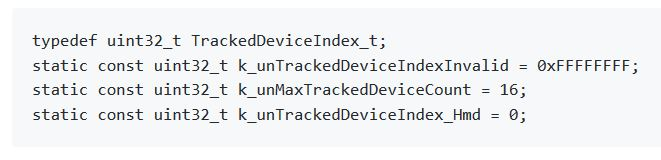
\includegraphics[width=10cm, height=3cm]{ivrsystem}}

	\caption{System interface \cite{openVR_fn_images} \label{fig:ivrsys}}
\end{figure}

Apart from the Head mounted Display there can be 15 other devices that can be active at any given time. This constant is stored as k\_unMaxTrackedDeviceCount.This number was determined arbitrarily it has nothing to do with hardware capabilities. 

Each tracked device has a class that is one of:

\begin{itemize}
	\item \textbf{TrackedDeviceClass\_Invalid} - There is no device at this index
	\item \textbf{TrackedDeviceClass\_HMD} - The device at this index is an HMD
	\item \textbf{TrackedDeviceClass\_Controller} - The device is a controller
	\item \textbf{TrackedDeviceClass\_TrackingReference} - The device is a camera, Lighthouse base station, or other device that supplies tracking ground truth.
\end{itemize}

\subsection{IVRChaperone}
The IVRChaperone namespace provides access to chaperone soft and hard bounds. Some of the accessors defined are

\begin{itemize}
	\item \textbf{GetPlayAreaSize} - to get the width/depth of the Play Area in meters.
	\item \textbf{GetPlayAreaRect} - is a rectangle which defines clear VR space from floor to ceiling where the player is.Required reachable interactions is kept in this space. 
	\item \textbf{GetCalibrationState} - Calibration state determines the state of base stations. If they are moved, this function may need to be polled until the state returns true; 
\end{itemize}

\subsection{IVRCompositor}

The IVRCompositor interfaces is used to provide access to the Compositor subsystem. The main objectives of this interface is to take care of distortion, prediction, synchronization and other subtle issues that can be a challenge by adjusting images to get a great VR experience.

Applications call WaitGetPoses to get the set of poses used to render the camera and other tracked objects, using the info giver by IVRSystem render the left and right eyes as normal and finally for Compositor to display in its own window submit undistorted textures.

General game loop algorithm goes like shown in Fig. \ref{fig:ivrcomp}.

\begin{figure}[H]
	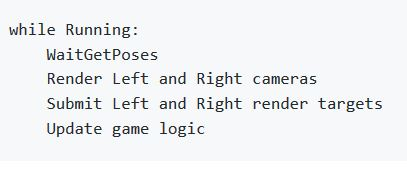
\includegraphics[width=8cm, height=3cm]{ivrcompositor} 
	\centering
	\caption{ Game loop algorithm for VR  \cite{openVR_fn_images} \label{fig:ivrcomp}}
\end{figure}

\subsection{IVROverlay}

The IVROverlay interface has functions which allows the calling application to control each overlay on their presentation, what they contain and receiving events. It is used to draw 2D images over 3D scene regardless of the application running.

To receive events, set attributes and render into the overlay a unique handle VROverlayHandle\_t is used for each overlay. In the circumstances where an overlay is not known or is otherwise invalid the handle will be equal to k\_ulOverlayHandleInvalid.

\subsection{IVRRenderModels}

The IVRRenderModels interface provides access to 3D models related to the attached hardware. Wherever possible these models reflect the actual physical appearance of the devices.

This interface contains the following functions:

\begin{itemize}
	\item \textbf{LoadRenderModel}- This function is expected by the API to be called during the start up and if the status of the device is changed to connected or disconnected. Calling this function every frame will hurt the performance. It loads and returns a render model for use in the application. The resulting render model stays valid until VR\_Shutdown() is called or until FreeRenderModel() is called. The method returns false if the model could not be loaded.
	
	\item \textbf{FreeRenderModel}-	Frees a previously returned render model.
	
	\item \textbf{GetRenderModelName}- Returns the name of the Nth render model that is provided by the OpenVR runtime. A number between 0 and the return value of GetRenderModelCount()-1 is the provided index. It is not the same as tracked device index. 
	
	\item \textbf{GetRenderModelCount}- Returns the number of render models provided by the OpenVR runtime.
	
\end{itemize}

\subsection{IVRScreenshots}
 To share and view screentshots in areas such as VR dashboard, Steam and other display applications IVRScreenshots interface is used.

Formats such ascubemap,stereo panoramic and mono panoramic are supported.
The most common screenshot that is a stereoscopic view stored as a side-by-side image.

The vr::IVRScreenshots interface provides the following functions:

\begin{itemize}

	\item RequestScreenshot
	\item HookScreenshot
	\item GetScreenshotPropertyType
	\item GetScreenshotPropertyFilename
    \item UpdateScreenshotProgress
    \item TakeStereoScreenshot
	\item SubmitScreenshot
	
\end{itemize}

\subsection{Other General Functions}

\begin{itemize}
	\item \textbf{IsHmdPresent()} - 
	If we want to check whether the HMD is present but not responding, this method is used. VR\_Init() may return NULL for various reasons for those cases this method is used to create a distinction whether device is not responding or not present as all.
	
	\item \textbf{IsRuntimeInstalled()} - 
	Returns true if the OpenVR runtime is installed on the system.
	
	\item \textbf{RuntimePath()} - 
	Returns location where the OpenVR runtime is installed.
	
	\item \textbf{GetVRInitErrorAsSymbol()} - This function is used to return enum value of EVRInitError as a string. It can be called any time, regardless of whether the VR system is started up.
	
	\item \textbf{GetGenericInterface()} - Requests an interface by name from OpenVR. It always return NULL if VR\_Init() has not been called successfully. If the interface is not found it will return NULL and pass back an error in peError. 
	
	\item \textbf{IsInterfaceVersionValid()} - 
	Depending on the installed runtime based on name and version returns boolean.
	
\end{itemize}

\section{"Hello Virtual World"}


To comprehend how to implement the openVR API we took a close look at the samples provided in the openVR source code. Particularly, they provided an example called "hellovr" which represents the basics of getting the headset up and running. This basic example took them ~2000 lines of code which is significantly larger than typical hello world examples in programming languages and gives you an idea about the complexity of implementing VR. It consisted of 3D cubes rendered along every direction to some extent and the controller acting as a laser pointer. The calls are being made to the HMD through the header file $"openvr_api.h"$. All the components are first initialized and information is received from tracked devices. Main loop consists of two functions, one is for rendering frames and the other is to receive and handle inputs. 

In the render function texture for each eye is made and pose for the HMD is updated along with three rendering tasks for controller axes, stereo targets which makes scenes for each eye, and a companion window. The call structure for Open VR is shown in Fig. \ref{fig:openvr_1}.

\begin{figure}[t]
	\includegraphics[width=9cm, height=5cm]{openvr_1} 
	\centering
	\caption{Open VR call structure \label{fig:openvr_1} \cite{openVR_fn_images}}
\end{figure}

When a pose update is request in the example, it calls a function that gets the poses for all tracked objects. Fig. \ref{fig:hellovrfn} shows the query for the poses, the storing of the types of tracked objects, and the saving of the pose of the HMD to a variable for later use. 
	

	\begin{figure}[h]
		\noindent
		\centering{\hspace{-2.5 ex}
			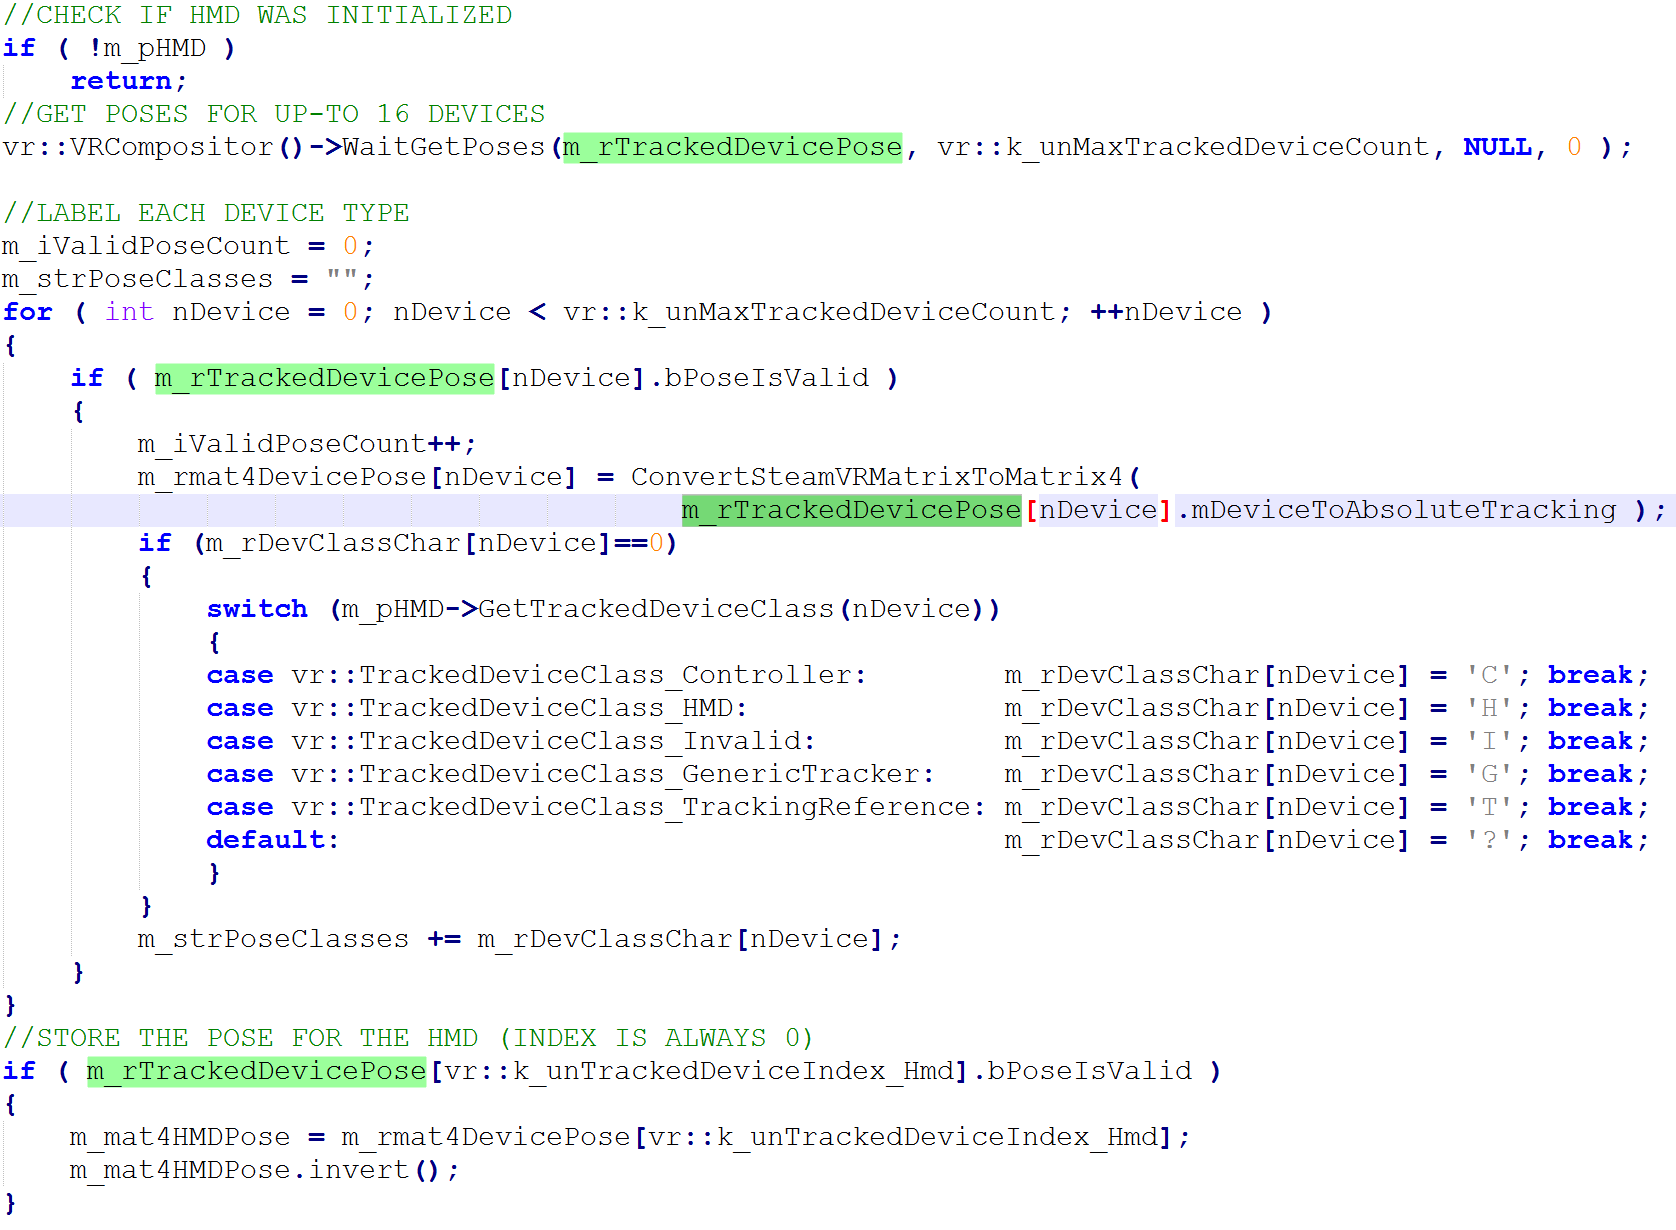
\includegraphics[height=9cm,width=11cm]{updateHMD_ALEX} }
		
		\caption{Update Head Mounted Display Matrix pose \label{fig:hellovrfn}
		}
	\end{figure}
	


\begin{figure}[h]
	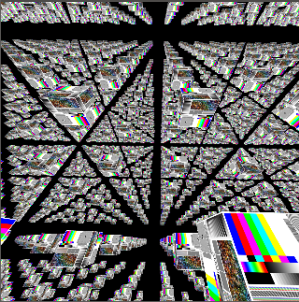
\includegraphics[width=8cm, height=5cm]{hellovr} 
	\centering
	\caption{Hello VR example \label{fig:hellovr} \cite{hello_ovr_images}}
\end{figure}


Upon running the Hello VR solution the screen looks as shown in Fig. \ref{fig:hellovr}. It shows rendering of 3d cubes along each axis inside a fixed volume. 
 
\section{Super Mario HD}

\begin{figure}[h]
	\noindent
	\centering{\hspace{-8 ex}
	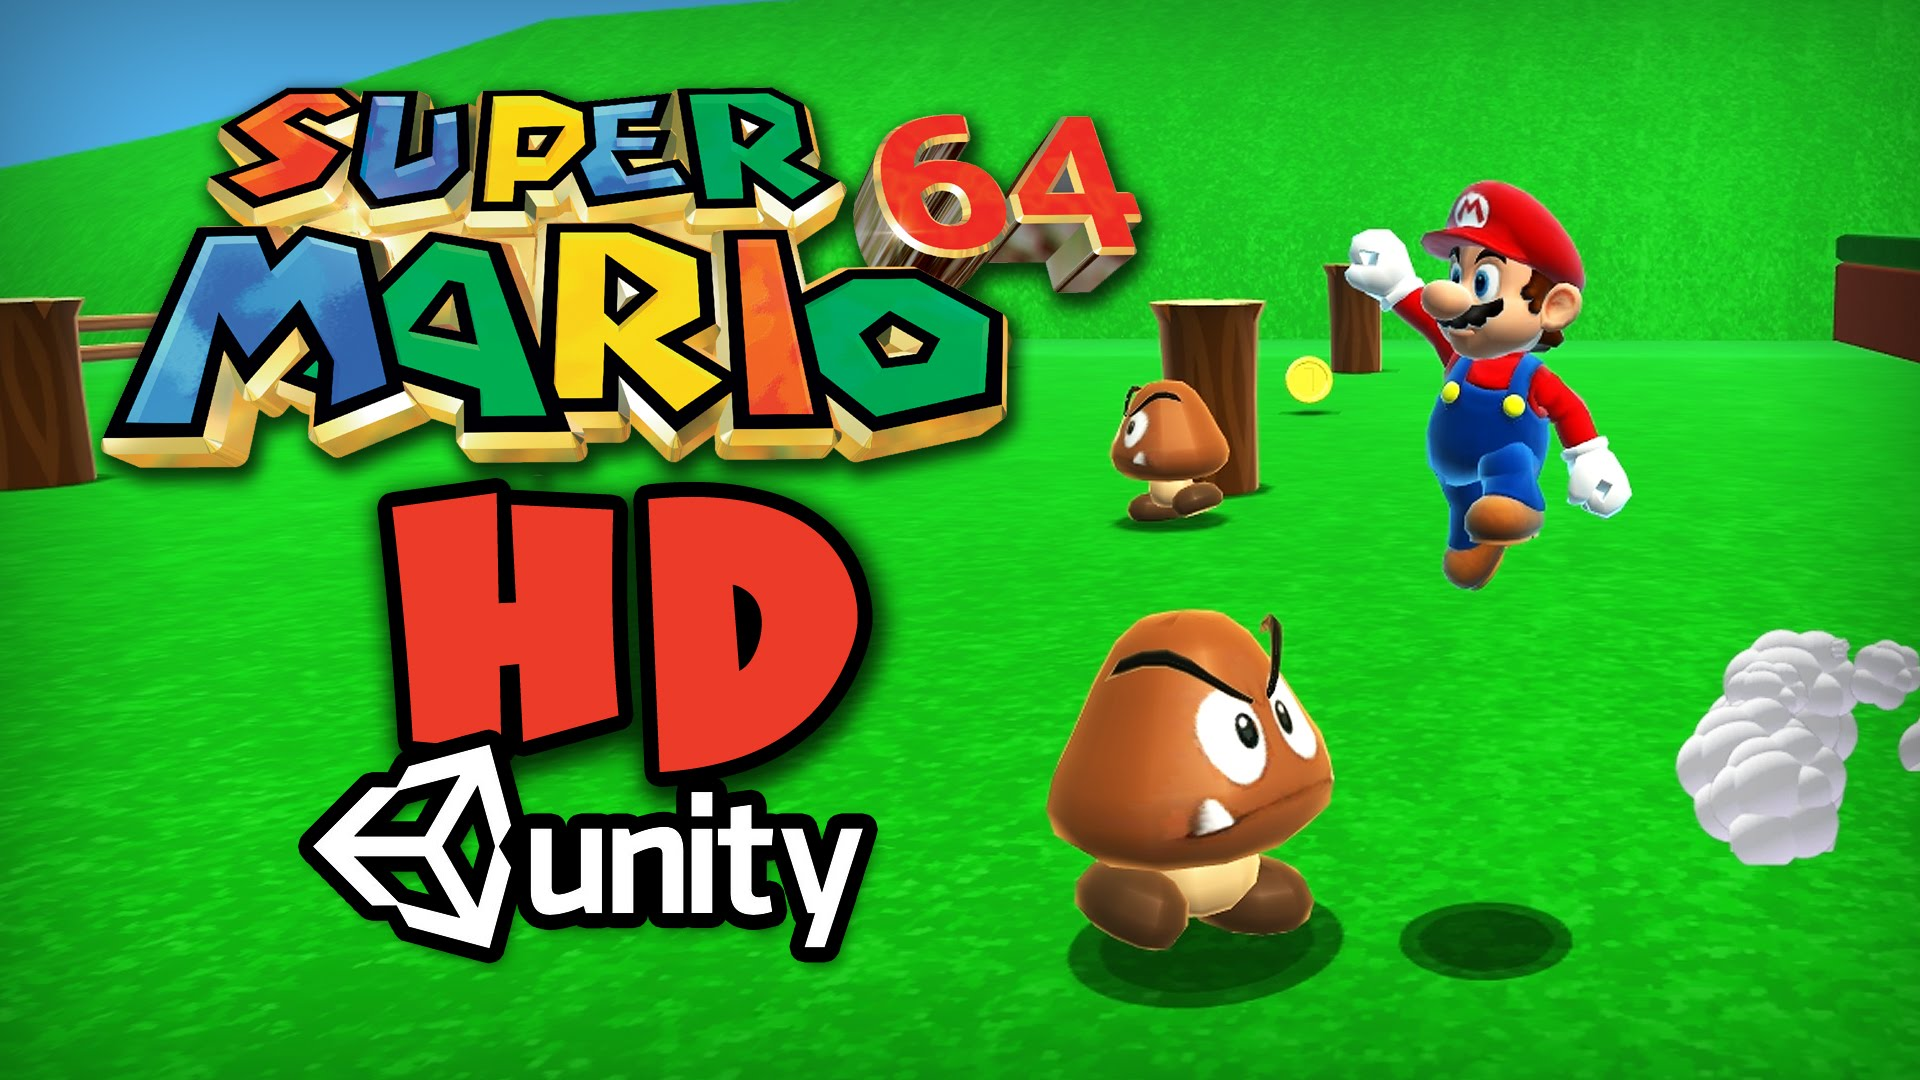
\includegraphics[width=10cm]{Mario64Header}}
	\caption{Mario 64 HD (Unity)\cite{mario_header} \label{fig:mario}}
\end{figure}

By far, Super Mario HD\cite{fig:mario} was the easiest game to implement virtual reality. Since this game was built using the Unity engine, we were able to utilized the open-VR asset from the assets store directly. This asset took care of all of the complex and annoying parts of implementing the initialization and rendering to the VR system. 

We modeled our VR implementation after the game Lucky's Tale. This game is a standard platforming game with VR being utilized as a way to control the camera view in a more natural manner.  A video showing the game play of our implementation and discussion of future work can be found in Figure \ref{Mario_Gameplay}.


\begin{figure}[h!]
	\noindent
	\centering{\hspace{2 ex}
		\includemedia[
		width=1.1\linewidth,height=0.61875\linewidth,
		activate=pageopen,
		flashvars={
			modestbranding=1 % no YT logo in control bar
			&autohide=1 % controlbar autohide
			&showinfo=0 % no title and other info before start
			&rel=0 % no related videos after end
		}]{}{http://www.youtube.com/v/A2wZEr1y0gA}
		\caption{Super Mario HD VR Demo and Future Work Discussion }
		\label{Mario_Gameplay}}
\end{figure}
\ref{fig:quake}.

Unity VR lets you target virtual reality devices directly from Unity, without any external plug-ins in projects. It provides a base API and feature set with compatibility for multiple devices. It has been designed to provide forward compatibility for future devices and software. The VR API surface is minimal by design, but will expand as VR continues to grow.


By using the native VR support in Unity, you gain:
\begin{itemize}
\item Stable versions of each VR device
\item A single API interface to interact with different VR devices
\item A clean project folder with no external plug-in for each device
\item The ability to include and switch between multiple devices in your applications
\item Increased performance (Lower-level Unity engine optimizations are possible for native devices)
\end{itemize}

\subsection{API Integration}
Unity provides natural integration with open-VR which can be enabled by checking the "Virtual Reality Support" option.

\begin{figure}[h]
	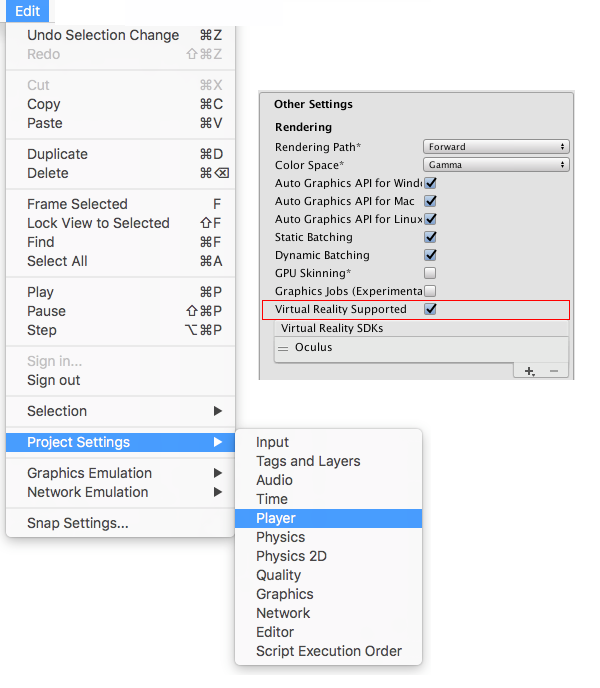
\includegraphics[width=8cm, height=8cm]{unity} 
	\centering
	\caption{Unity 3D enabling VR \label{fig:unity} \cite{unity}}
\end{figure}


\subsection{Rendering Integration}

All Cameras in your Scene are able to render directly to the head-mounted display (HMD). View and Projection matrices are automatically adjusted to account for head tracking, positional tracking and field of view. The integration can be done as shown in Fig. \ref{fig:unity}.

We made the main camera a child of Mario so it follows his actions. It is possible to disable rendering to the HMD using the Camera component’s stereoTargetEye property. Alternatively, it is possible to set the Camera to render to a Render Texture using the Target Texture property.
Using the stereoTargetEye property to set the Camera to only render a specific eye to the HMD. This can be achieve by adding two Cameras to the Scene: one targeting the left eye, the other targeting the right eye. Set layer masks to configure what is sent to each eye. Since this game didn't need any special target texture rendering only one camera was configured.



\subsection{Tracking Integration}

Upon adding the prefabs provided by the open VR API the head tracking and the appropriate field of view (FOV) is automatically applied to the Camera if the device is head-mounted. It is possible to manually set the FOV to a specific value, but it cannot set the Camera’s transform values directly. For Mario we didn't need to set the field of view manually.

Unity automatically applies Head tracking and positional tracking, so that before the frame is rendered the position and orientation most closely matches user’s position and orientation. This gives a good VR experience, and prevents the user from experiencing nausea.

\subsection{Controller Integration}

For this project we didn't integrate the Vive controllers but used the X-Box One controller which came integrated with the game. It made more sense to control the character via joysticks from a third-person perspective.

\subsection{Future Work}

Upon testing we found out that users felt nauseated upon long use. We will be working on camera angles to fix this problem. Another approach that might be taken is to have a fixed camera around certain locations when Mario moves. The second approach reduces the immersion of users but their experience is less nauseating. We made a prototype of this form of play by making "God mode" through which player can experience the game via a high camera angle.




\section{FreeSpace 2}


\begin{figure}[h]
	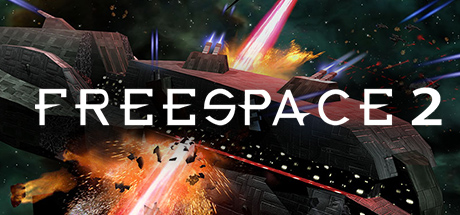
\includegraphics[width=10cm]{FreeSpaceHeader} 
	\centering
	\caption{FreeSpace 2\cite{freespace_header}}\label{freespace_header}
\end{figure}

We used an open source version of FreeSpace 2 as the base code\cite{free_space_2_original_source} for our virtual reality integration. This code was written in C++ and used many C++ programming techniques that we were not familiar with. Such techniques, were the way the somehow handles the OpenGL rendering using wrappers of pointers to functions.

The target we set for FreeSpace 2\ref{freespace_header} was to render to the headset and use the orientation tracking to point the ship in the direction you are looking. We were successful in doing those tasks, though due to time limitations were not able to work out bugs with rendering that cause double vision in the headset for some of the textures. A video showing the game play of our implementation and discussion of future work can be found in Figure \ref{FS2_Gameplay}.


\begin{figure}[h!]
	\noindent
	\centering{\hspace{2 ex}
		\includemedia[
		width=1.1\linewidth,height=0.61875\linewidth,
		activate=pageopen,
		flashvars={
			modestbranding=1 % no YT logo in control bar
			&autohide=1 % controlbar autohide
			&showinfo=0 % no title and other info before start
			&rel=0 % no related videos after end
		}]{}{http://www.youtube.com/v/cvg3PfHSzaw}
		\caption{FreeSpace 2 VR Demo and Future Work Discussion }
		\label{FS2_Gameplay}}
\end{figure}


\subsection{API Integration}
Calls to the SDK were made through the header file $"openvr\_api.h"$. The intergeneration of the API into the source code was painful due to the complexity of the project and being unfamiliar with Make files. This probably took us 30\% of the effort to get the API calls to work correctly. 

Once the API calls were working, we encapsulated most of the API calls into a object called VR.cpp. This helped keep the code somewhat cleaner and allowed us to directly borrow and modify many of the helper functions found in the hello world example.

\subsection{Rendering Integration}
Integration of rendering was challenging for this game compared to Quake. OpenVR requires textures to be drawn for each eye and then submitted to the headset API and this game does not draw directly to textures. Additionally, the OpenGL calls made by the game were not easily accessible in the code. All we ended up having to use the glCopyTexSubImage2D OpenGL function to copy the current data into our texture for the headset. Figure \ref{freespace_render} shows the code used for the left eye. 

\begin{figure}[h]
	\noindent
	\centering{\hspace{-10 ex}
		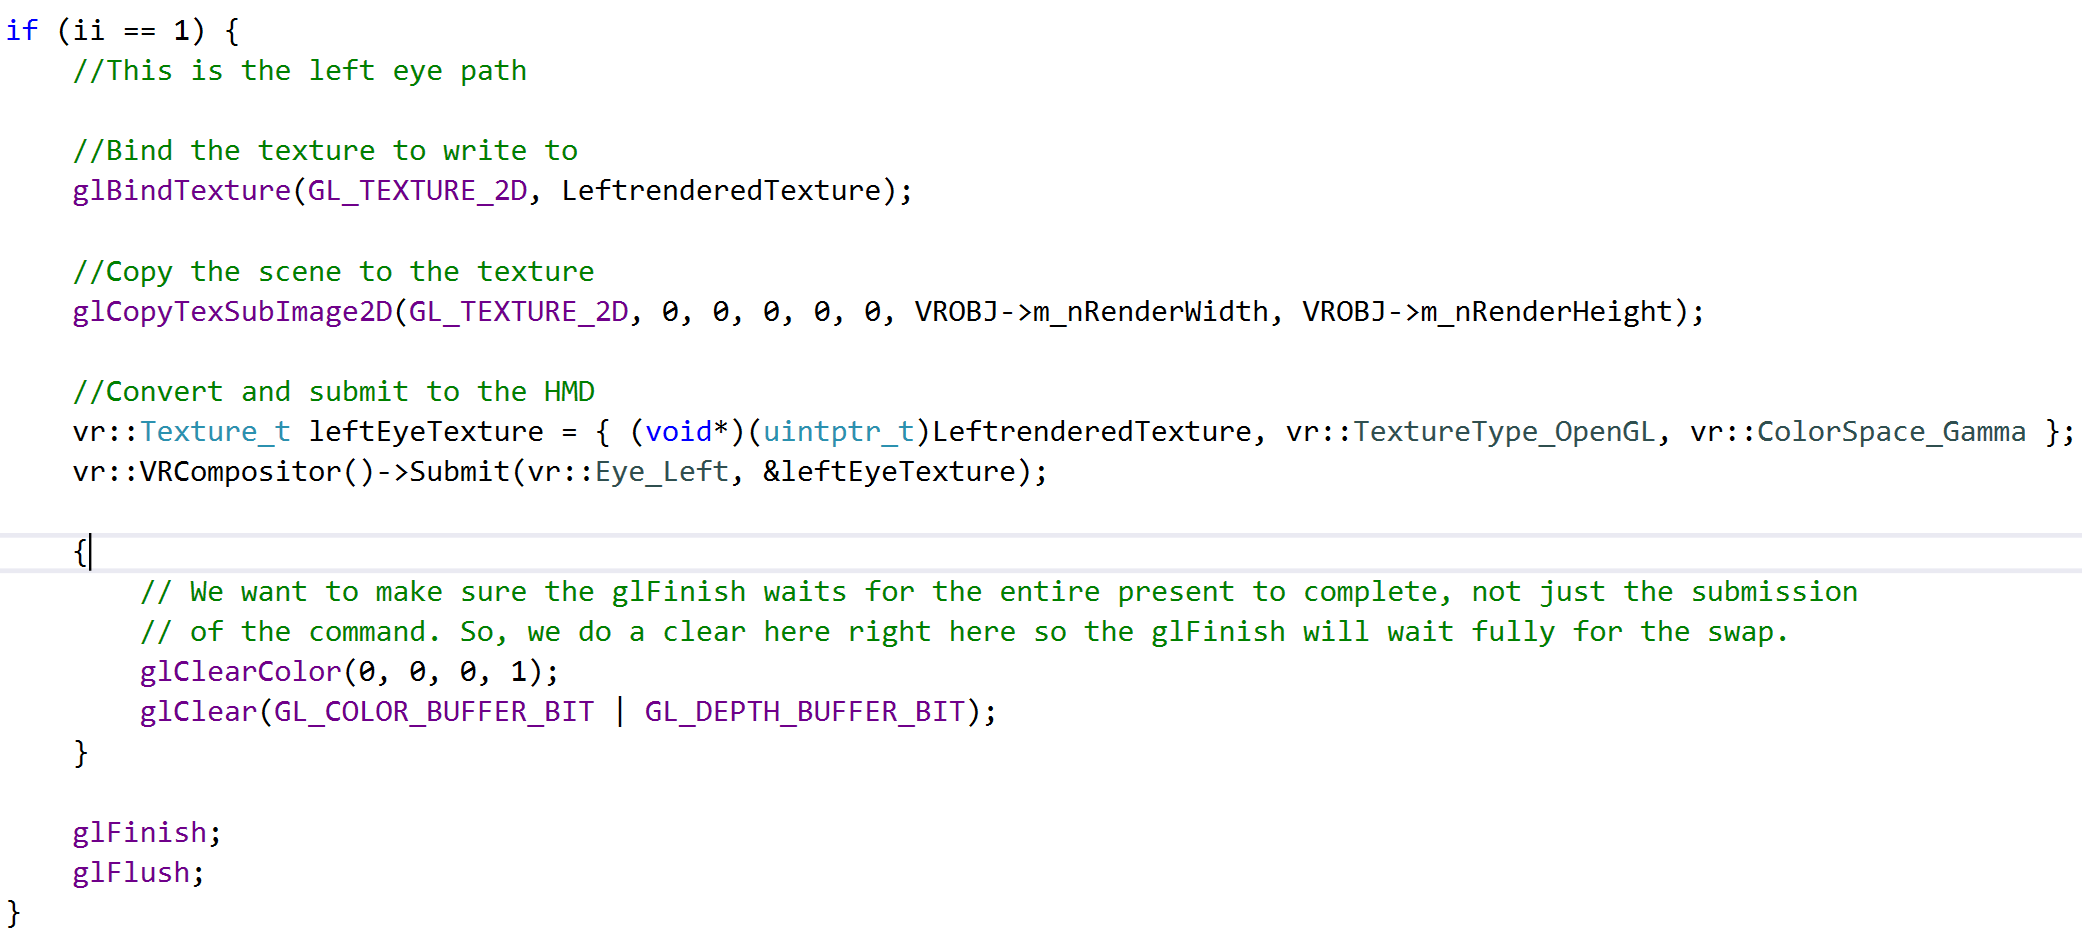
\includegraphics[height=6cm,width=10cm]{freespace_rendering} }
	
	\caption{Example OpenGL code for FreeSpace 2.  \label{freespace_render}
	}
\end{figure}

Another notable things about the Rendering is that we needed to query the OpenVR API to get each eye projection matrix, resolution, and eye offsets. We applied those values directly to the rendering chain which made all of the 3D rendering look correct. The 2D rendering such as the textures for the HUD or the Nebula did not offset correctly and we did not resolve that before the end of the project. This 2D rendering issue also required us to turn of rendering of asteroids and stars to make the game potable. 

\subsection{Tracking Integration}
Integration of tracking was straight forward. We updated the pose of the HMD every iteration of the game loop and was able to directly use the rotation matrix provide to set the orientation of the camera and player objects in the code. 


\subsection{Future Work}
We do not plan to continue working on this game or releasing this to the public. We believe that it would be difficult to resolve the 2D rendering issues without a large rework of the rendering chain. 

If we were going to continue work on this, we would first integrate a gamepad or motion controller so you do not need a mouse and keyboard. This would allow for a more comfortable experience for the user. We then would work on fixing the 2D rendering. With those two items complete, this game would be ready for release to the general public.  


\section{Quake}

\begin{figure}[h]
	
\includegraphics[width=10cm]{QuakeHeader} 
	\centering
	\caption{Quake 1\cite{quake_header} \label{fig:quake}}
\end{figure}

 Quake is built in C, the version we used is "Quakespasm" it is a modification of original Quake game source code which adds extra features like Graphics, No need for DOS or a DOS-emulating platform, SDL (Simple Direct media Layer) Based executable, Dynamic lights, Model interpolation, and Support for 64bit systems. The particular version were were using had Oculus Rift integration which was used to only aim using the HMD. Our target was  to successfully render to a head-mounted display (HMD), receive tracked input and handle controller/other events sent by the HTC Vive system. Optimally we wanted to be able to independently move the player and the gun, but only succeeded with moving the camera independently from the gun with the controller providing orientation for the gun.
 
 In the end we had two version of the VR integration. Version A had orientation tracking only for the camera (based on the HMD) and the gun (based on the controller) with all the movements being relative to the gun's pointing. Version B had position tracking for the camera(based on the HMD) and orientation tracking for the gun(based on the controller) with all of the movements being relative to the camera pointing. By far, Version A was a superior experience. 
 
  A video showing the game play of our implementation and discussion of future work can be found in Figure \ref{Quake_Gameplay}.


\begin{figure}[h!]
	\noindent
	\centering{\hspace{2 ex}
		\includemedia[
		width=1.1\linewidth,height=0.61875\linewidth,
		activate=pageopen,
		flashvars={
			modestbranding=1 % no YT logo in control bar
			&autohide=1 % controlbar autohide
			&showinfo=0 % no title and other info before start
			&rel=0 % no related videos after end
		}]{}{http://www.youtube.com/v/xkSN3_J4Cbg}
		\caption{Quake VR Demo and Future Work Discussion }
		\label{Quake_Gameplay}}
\end{figure}
 \ref{fig:quake}.


\subsection{API Integration}
Calls to the SDK were made through the header file $"openvr\_capi.h"$. Unlike with FreeSpace 2, there was no example supplied of the API calls for the C API. Luckily we were able to find someone who re-write the original example using the C API (CITE) and we were able to utilize this for most of our work . Added the API to the code base was a lot simpler because we added the required libraries and header file directly in Visual Studio. This was possible due to the game being significantly less complex than FreeSpace 2 and we did not need to work with Make files.      

We were required to rip most of the Oculus SDK code out of the source so we could replace it with the OpenVR code. The benefits we got from this is that we did not need to make any new user interfaces since we could the onces developed for the Oculus SDK.

We ended up encapsulating most of the required API calls into a VR.c object. Like with FreeSpace 2, it helped keep the code somewhat cleaner and allowed us to directly borrow and modify many of the helper functions found in the hello world example.
 
\subsection{Rendering Integration}

Integrating HMD rendering in Quake was less difficult than with FreeSpace 2. A lot of the changes in the flow of the rendering chain was already complete due to the previous integration of Oculus Rift. As with FreeSpace2 we needed to provide the correct project, eye offset. This information was queried from the API at the beginning of the VR initialization. 

Figure \ref{quake_rendering} shows some of the rendering chain we implemented. First we calculate the updated pose for each eye by multiplying the each respective eye offset matrix with the HMD pose matrix. We store the updated projection matrix as well (in theory this could change during game play). We then render the scene with that information and store the textures in a OpenVR friendly format. This gets submitted for both eyes and then we blight the right eye's framebuffer to the backbuffer so we can draw to a monitor. 

An interesting thing to note is that the Oculus SDK actually handles the generation of a mirror texture for the monitor for you. OpenVR is more low level implementations when it comes to functions like that. 

\begin{figure}[h]
	\noindent
	\centering{\hspace{-8 ex}
	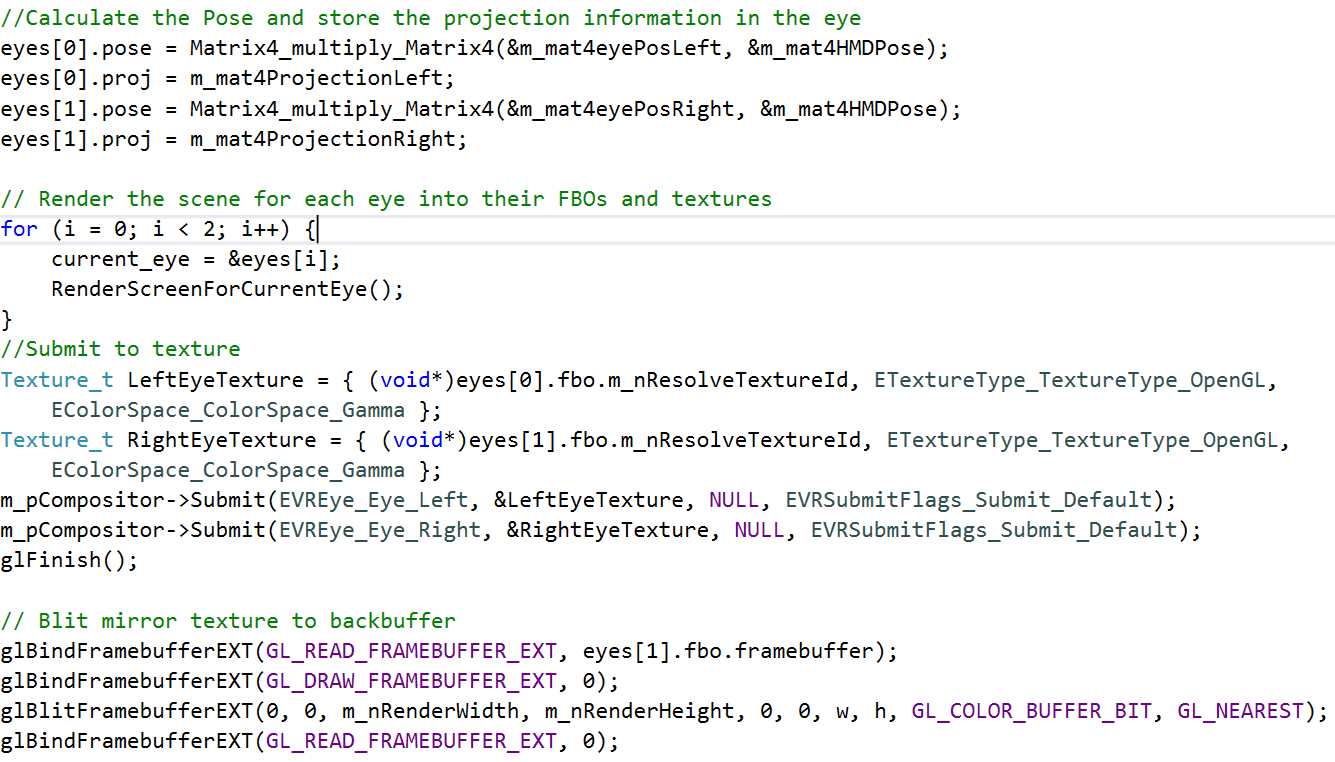
\includegraphics[width=10cm, height=7cm]{quake_rendering} }
	\centering
	\caption{Example of rendering path for Quake}\label{quake_rendering}
\end{figure}

Version A of our code throws out the translational information of each eye, while version B keeps it to use as an offset. 

\subsection{Tracking Integration}

All of the pose information coming in from the tracking is stored as rotational matrices. Quake, on the other hand, uses only yaw, pitch, and roll. There is an inherent issue with yaw, pitch, and roll coordinate frames when you are truly able to move in all orientations. This effect is called gimbals lock and may be apparent when you look how the gun's reacts to changes in roll (see video).

Similar to FreeSpace 2, we updated the pose of the HMD every iteration of the game loop and was able to directly use the rotation matrix provide to set the orientation of the camera. Additionally we need the orientation of the controller so we added an extra section of code at the end of pose update function (Fig. \ref*{fig:hellovrfn}) to store the controller information. This code is shown in Figure \ref{controller_pose}. We then took the rotational matrices and converted it to yaw, pitch, and roll so we could feed it directly to as the gun's aim point. 

\begin{figure}[h]
	\noindent
	\centering{\hspace{0 ex}
		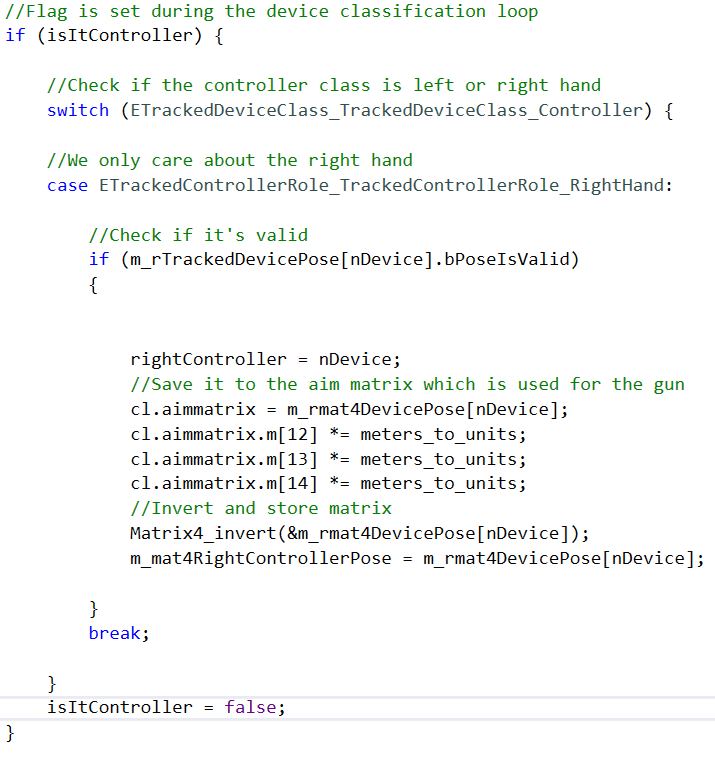
\includegraphics[width=10cm, height=10cm]{controller_pose} }
	\centering
	\caption{Example of saving the controller pose}\label{controller_pose}
\end{figure}

\subsection{Controller Integration}
Controllers were used for movement, shooting and pausing the game. The trackpad works as a pad monitor for forward and backward motion of the player. The trigger button of the controller was used in shooting and the menu button paused the game which causes the options to appear. Since the game was adapted to work with oculus, the movement and hit detection was attached to the controller. We tried unwinding this system to make controllers and HMD work separately. The game play was not smooth in this case. The players had to look in the direction in which they wanted to go, which was uncomfortable. The second approach was to move in the direction the controller was pointing, this lead to a better gameplay design as a whole. 

\begin{figure}[h]
	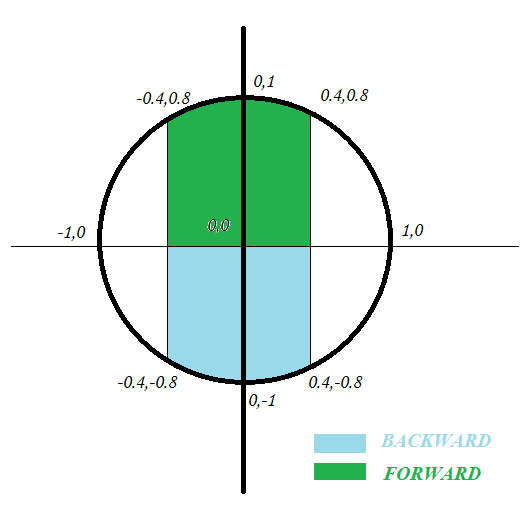
\includegraphics[width=8cm, height=8cm]{controller} 
	\centering
	\caption{Coordinate system in trackpad \label{fig:contr}}
\end{figure}

Events in the controllers were tracked to notify the inputs in realtime. The handling of the trackpad and controller buttons where entirely separate in the API. Trackpad sensors recorded touch of the finger/thumb in x/y coordinates which ranged form 0 to 1 in every direction as shown in Fig. \ref{fig:contr}. The events from the trackpad depends on the axis of the controller and events are received through GetControllerState function as shown in  Fig. \ref{fig:contr1}

\begin{figure}[h]
	\noindent
	\centering{\hspace{0 ex}
	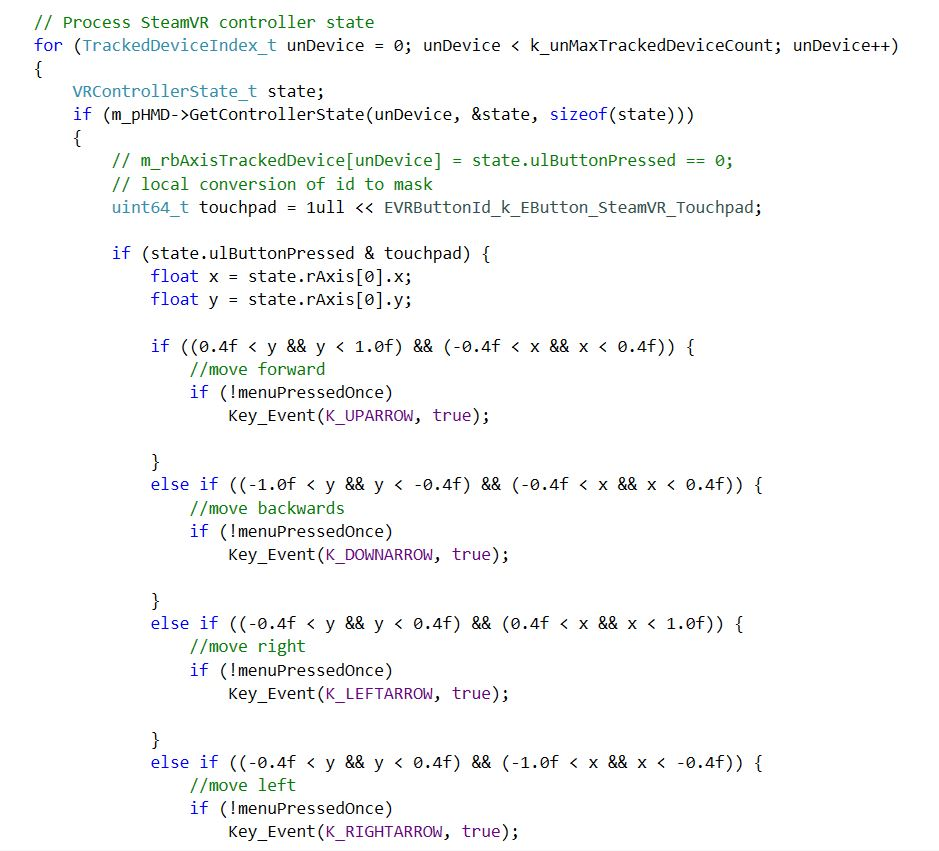
\includegraphics[width=10cm, height=10cm]{controllerTrackpad}}
	\centering
	\caption{Controller state handler \label{fig:contr1}}
\end{figure}

If the event received is button down, the event is type casted to VREvent\_Controller\_t pointer and looped to check which buttons are in the down state. Same thing is done for controller button up events as shown in Fig. \ref{fig:contr2} . Here when the trigger button is pressed we are sending the SDL event K\_MOUSE1 to simulate first mouse button clicked which is mapped to shooting in the game.

\begin{figure}[H]
	\noindent
	\centering{\hspace{0 ex}
	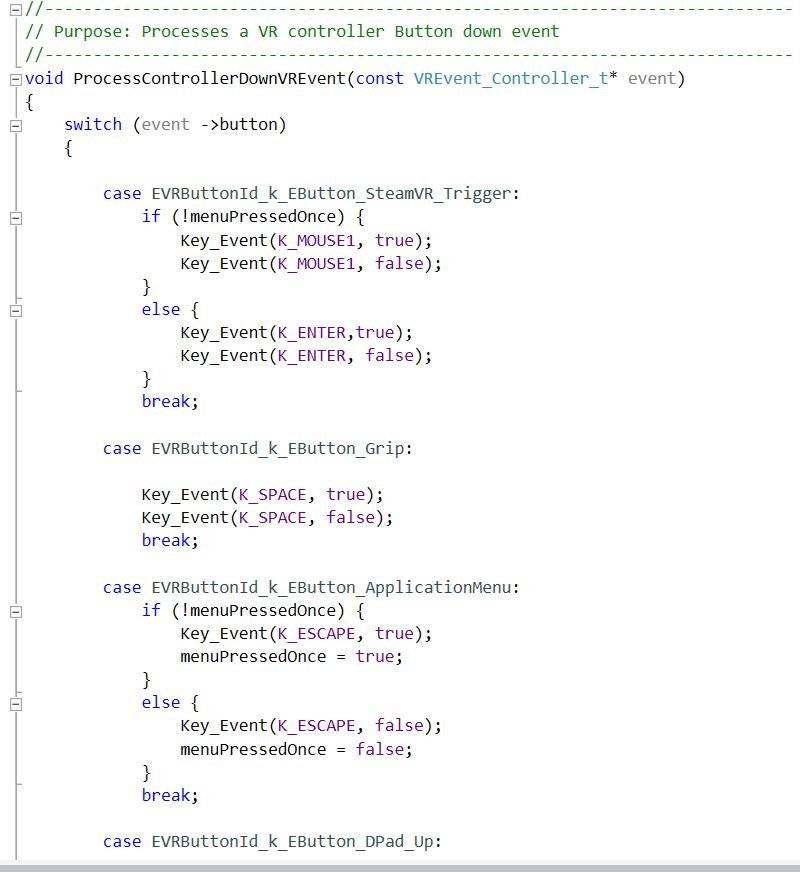
\includegraphics[width=9.5cm, height=9.5cm]{controllerButton}} 
	\centering
	\caption{Controller button down event handler \label{fig:contr2}}
\end{figure}

\subsection{Future Work}
We may be releasing version A of the code as is to the public after this course. We believe that the code is fun enough and usable enough for the general public. We also are considering continue our work on the code base to bring in positional tracking of both the camera and the gun, as well as, adding in teleportation. 

\section{Project Takeaways}

This project has been a great experience for us to learn some of the difficulties and requirements to integrate virtual reality into games. We have a couple take aways we would like to highlight that may be useful for anyone else who goes down this path. 

The first takeaway is that integrating VR into existing games is not always practical. This is because during the development of games, certain assumptions may be made that makes sense for 2D monitors but does not make sense when you have complete 6 degrees of freedom. These assumptions could be made to make the game run faster or the coding easier. It may be better to write a game from scratch than to hack in virtual reality components. 

The other takeaway is to use Unity or Unreal Engine where possible. The integration with VR is simple to use, and you do not need to worry about handling a lot of the background calculations your self. There is also a lot of resources for Unity and VR that just don't exist for direct API calls in C or C++. 



\begin{thebibliography}{10}
	
				
	\bibitem{openVR_images} 
	\textbf{Image:}http://www.valvetime.net/threads/using-unity-at-valve-vision-summit-2016.253857/
		
			\bibitem{openVR_fn_images} 	
			\textbf{Image:}https://github.com/ValveSoftware/openvr/wiki/API-Documentation
			
			\bibitem{hello_ovr_images} 
			\textbf{Image:}https://kheresy.wordpress.com/2016/12/12/openvr-opengl/
			
			\bibitem{unity}
			\textbf{Link:}https://unity3d.com/learn/tutorials/topics/virtual-reality
			
			\bibitem{mario_header}
			\textbf{Link:}https://celofans.mx/wp-content/uploads/2015/03/mario64.jpg 
			\bibitem{freespace_header}
			\textbf{Link:} http://cdn.akamai.steamstatic.com/steam/apps/273620/header.jpg\hspace{1cm} ?t=1447360124	
			
			\bibitem{quake_header}
			\textbf{Link:}https://camo.githubusercontent.com/944c03fe666eacc0cdfdcf\hspace{1cm} 1331d8973293386444/687474703a2f2f7777772e67616d6572616e782e6\hspace{1cm} 36f6d2f696
			d616765732f757064617465732f313239343035333236395f7\hspace{1cm} 175616b655f6670732e6a7067
			
			\bibitem{free_space_2_original_source}
			\textbf{Source Code:} https://github.com/scp-fs2open 
			
			\bibitem{quake}
			\textbf{Quake repo:}https://github.ccs.neu.edu/buildingagameengine/Quakespas\hspace{1cm}mOpenVR.git
			
			\bibitem{freespace}
			\textbf{Freespace 2 repo:}https://github.ccs.neu.edu/buildingagameengine/fs2op\hspace{1cm}enVR
			
			\bibitem{mario}
			\textbf{Mario repo:} https://drive.google.com/file/d/0B6qEE4W2IQKcX0NLW\hspace{1cm}EhuR2VDQUE/view

\end{thebibliography}





\end{document}




   
